\documentclass[senior,final,11pt]{iscs-thesis}
\usepackage[dvipdfmx]{graphicx}
\etitle{A Method of Improving QoS:  Explorations of the Possibility of Function Combinations in Service Compositions}
\jtitle{品質改良のアプローチ:機能のぶれを許すサービス合成}
%
\eauthor{Ziyuan Wang}
\jauthor{王子源}
\esupervisor{Shinichi Honiden}
\jsupervisor{本位田真一}
\supervisortitle{Professor} % Professor, etc.
\date{February 9, 2016}
%-------------------
\begin{document}
\begin{eabstract}
There is a growing need for web service providers to develop customised and flexible web services as quick as they can. One way to satisfy this demand is to utilise service compositions, which provide a method of consolidating several services to a richer service. Because of the uncertainty in the feasibility of the functional and QoS requirements, it is not guaranteed that service compositions succeed with suitable solutions.

One way to satisfy the given requirements is to control the given two kinds of requirements. There have been studies on methods of optimising the QoS with fixed functional requirements. However, the search space in that case is limited, which would possibly not include service compositions with better QoS whose functions are slightly different from the required one. Therefore, I focus on the possibility of improving the QoS by compromising on functions or exploring the possibility of function combinations. This enables better advice of service compositions to users. In this article, I propose a method of efficiently searching different possibilities to support users to balance functional requirements and QoS requirements.
\end{eabstract}
\begin{jabstract}
近年,ウェブサービスプロバイダーにとって,ユーザーの好みに合わせた,柔軟なウェブサービスを短時間で作る必要性が増してきている.そのために,よく使われている手法として,複数のサービスを一つにまとめてより高機能なサービスを作るサービス合成と呼ばれる手法がある.サービス合成において,入力として受け取る機能や品質に関する要求を必ず満たせるとは限らないという問題がある.

機能と品質の両方を達成するために既存研究で提案されている手法として,その片方を固定して保証し,もう片方を最適化するというものがある.しかし,この手法では,機能を固定するために,探索空間が限られているため,
要求された機能に妥協を許した場合に品質が大きく高まるような合成を見逃す可能性がある.よって,本論文では,ユーザーが高品質の合成を見つけることがより容易になるよう,機能を妥協し,要求された機能と少しのぶれを許すことで探索空間を増やすことによるQoSの最適化の可能性について議論した.本論文では,ユーザーが機能要求と品質要求のバランスを取れるように効率的に様々な合成の可能性を探索する手法を提案した.

\end{jabstract}
\maketitle

\begin{acknowledge}
I appreciate Prof. Ishikawa's help in improving the structure of the paper.
\end{acknowledge}

\frontmatter 
\tableofcontents
%\listoffigures
%\listoftables 
%\lstlistoflistings
%-------------------
\mainmatter 

\chapter{INTREODUCTION}
Web service, service-based system, and service composition are significant.

%Web service:

%随着互\UTF{8054}网的迅猛\UTF{53D1}展和广泛\UTF{5E94}用,Web服\UTF{52A1}作\UTF{4E3A}部署在互\UTF{8054}网上的\UTF{7EC4}件,展\UTF{73B0}出良好的封装性、松\UTF{8026}合性以及跨平台性。越来越多的\UTF{5F00}\UTF{53D1}者将他\UTF{4EEC}做的serivce\UTF{53D1}布到个人网站或者\UTF{7C7B}似于amazon的平台,以期待\UTF{8BA9}\UTF{522B}人无\UTF{507F}或者有\UTF{507F}地使用,因此,Web服\UTF{52A1}成\UTF{4E3A}了人\UTF{4EEC}\UTF{5173}注的焦点。

%service-based system:

%service-based system 的主要目的 通\UTF{8FC7}\UTF{6784}筑一个通用的、与平台和\UTF{8BED}言无\UTF{5173}的技\UTF{672F}\UTF{5C42},使得各\UTF{79CD}不同平台上的\UTF{5E94}用系\UTF{7EDF}\UTF{95F4},\UTF{5B9E}施彼此的\UTF{8FDE}接和集成。
%其中,既有企業間の商取引を担う大規模なものから、也有単一の機能を持ったコンポーネント(ソフトウェア部品)まで、様々な規模・種類のものがある。

%service composition:
%\UTF{5355}一web service的\UTF{95EE}\UTF{9898}\UTF{95EE}\UTF{9898}%
%但是\UTF{5355}一的Web服\UTF{52A1}所提供的功能有限,因此需要把已有的Web服\UTF{52A1}\UTF{7EC4}合起来,生成\UTF{6EE1}足用\UTF{6237}需求的\UTF{7EC4}合服\UTF{52A1}。在服\UTF{52A1}\UTF{7EC4}合\UTF{8FC7}程中,如何根据用\UTF{6237}\UTF{8F93}入信息快速地找出相\UTF{5173}Web服\UTF{52A1}生成\UTF{7EC4}合服\UTF{52A1}成\UTF{4E3A}了服\UTF{52A1}\UTF{7EC4}合的\UTF{5173}\UTF{952E}\UTF{95EE}\UTF{9898}。
%做\UTF{4E3A}一\UTF{79CD}有效的解决方法,

%Service compositions are widely used in industry and research in order to create a functional richer loosely coupled service quickly. 

%service compostions的用途和\UTF{96BE}点
%service compositions 一般有\UTF{4E24}\UTF{79CD},一\UTF{79CD}是,没有workflow template做\UTF{4E3A}模版 ,重\UTF{89C6}能否得到一个可能的workflow,也就是一个可行的合成建\UTF{8BAE},而忽略non\UTF{FF0D}funtional (也就是qos)的好坏的planning algorithm。一\UTF{79CD}是将固定的workflow template作\UTF{4E3A}\UTF{8F93}入,重\UTF{89C6}最\UTF{4F18}化qos的selection algorithm。
%而在本\UTF{8BBA}文中,我\UTF{4EEC}主要研究能\UTF{591F}更精\UTF{786E}得到\UTF{7ED3}果的后者,基于 QoS 的 Web 服\UTF{52A1}\UTF{9009}\UTF{62E9}\UTF{95EE}\UTF{9898}。
\section{Background}

%因\UTF{4E3A}, 参与合成的service  一般具有不同 QoS 参数 ( 如\UTF{6267}行\UTF{65F6}\UTF{95F4}、服\UTF{52A1}\UTF{8D39}用、可用性、可 靠性、安全性、声誉等) 的候\UTF{9009}服\UTF{52A1},\UTF{8FD9}些候\UTF{9009}服\UTF{52A1}具有相似但又不尽相同的功 能属性和不同非功能属性 ,所以如何高效\UTF{52A8}\UTF{6001}地把\UTF{73B0}存的各\UTF{79CD} Web 服\UTF{52A1}聚合起来以形成新的\UTF{6EE1}足不同用\UTF{6237}的 功能需求 和 QoS需求 的\UTF{590D} \UTF{6742}服\UTF{52A1},是一件非常挑\UTF{6218}的事 。服\UTF{52A1}\UTF{9009}\UTF{62E9} 的\UTF{7ED3}果不\UTF{4EC5}直接\UTF{5173}系到服\UTF{52A1}能否成功\UTF{7EC4}合,而且\UTF{5BF9}\UTF{7EC4}合服\UTF{52A1}的\UTF{8D28}量有着至\UTF{5173}重要的影 \UTF{54CD}[1] 。

%A lot of existing studies on QoS-aware service composition.
%由此可\UTF{89C1},利用QoS(quality of service)\UTF{9009}\UTF{62E9}服\UTF{52A1}已成\UTF{52A8}\UTF{6001}Web服\UTF{52A1}\UTF{7EC4}合\UTF{5B9E}用化的\UTF{5173}\UTF{952E}技\UTF{672F}。目前,国内外的学者在基于QoS的\UTF{52A8}\UTF{6001}Web服\UTF{52A1}\UTF{7EC4}合方面已\UTF{7ECF}做了一些工作,(比如 \UTF{8C01} \UTF{8C01} \UTF{8C01} 之后在ralted work中再提起,或者就在\UTF{8FD9}里\UTF{8BA8}\UTF{8BBA}),但是他\UTF{4EEC}都\UTF{4EC5}\UTF{4EC5}探\UTF{8BA8}了将固定的funciton requirements作\UTF{4E3A}\UTF{8F93}入。

\section{Motivation}
%Fixed functional requirements -> may lose potential improvement of QoS, difficulty for users to properly define the functional requirements because of uncertainty of the feasibility of requirements given available services
%\UTF{8BA8}\UTF{8BBA}固定fun的不好 -->   它会\UTF{5BFC}致没法找到更好的qos

%当\UTF{4F60}\UTF{4E3A}了\UTF{6EE1}足\UTF{4F60}的目的 想出一个固定的functional requirement(固定功能,最\UTF{4F18}化qos),将它\UTF{8F93}入一个系\UTF{7EDF},\UTF{4F60}是没有\UTF{529E}法直\UTF{89C2}地判断它所得出的  workflow的QoS\UTF{503C}到底是\UTF{6EE1}足\UTF{4F60}目的(不是\UTF{4F60}的funcitonal requiremnet) 的全局最\UTF{4F18}的 \UTF{8FD8}是不是 。很有可能\UTF{4F60}的要求太\UTF{4E25}格了,\UTF{5BFC}致原本功能弱一点(但也\UTF{6EE1}足\UTF{4F60}目的)的workflow不在\UTF{4F60}的搜索空\UTF{95F4}内。又或者是\UTF{4F60}制定functional requirement太片面,没将\UTF{5B9E}\UTF{9645}上功能上超\UTF{989D}\UTF{6EE1}足\UTF{4F60}要求的function放入\UTF{4F60}的搜索空\UTF{95F4},\UTF{5BFC}致\UTF{4E27}失了找到    funciton也\UTF{5F3A}\UTF{8FC7}\UTF{4F60} QoS也\UTF{5F3A}\UTF{8FC7}\UTF{4F60}的 workflow。
%\UTF{6362}言之,\UTF{4F60}的目的 和\UTF{4F60}\UTF{9009}定的 functional requirement很可能有gap,而且\UTF{8FD9}个是不自\UTF{89C9}的并且之后也是不能很快\UTF{9A8C}\UTF{8BC1}的。我\UTF{4EEC}可以\UTF{8BB2}\UTF{4E24}个故事。
%第一个例子:
%web service providers want to create a service which use S1 or S2 as first service of workflow.
%service purpose: help user to rental a car for shopping
%if providers insist “can search any car” as input part of functional requirements, he will not find the best solution !

%第二个例子:
%s1: 在amazon\UTF{4E70}一\UTF{79CD}特殊的米 s2:在米的\UTF{4E13}\UTF{5356}店(网上)一\UTF{79CD}特殊的米
%service purpose: \UTF{4E70}相同\UTF{79CD}\UTF{7C7B} 价格最便宜的米
%由于制造者\UTF{4EC5}\UTF{4EC5}依靠自己的\UTF{7ECF}\UTF{9A8C} \UTF{89C9}得\UTF{4E13}\UTF{5356}店便宜,于是就\UTF{8BBE}定功能\UTF{4E3A}只能“\UTF{4E13}\UTF{95E8}\UTF{4E70}米”,将能\UTF{4E70}其他\UTF{4E1C}西的(比“只能\UTF{4E70}米”功能\UTF{5F3A}的)服\UTF{52A1}排除在搜索范\UTF{56F4}之外。\UTF{5B9E}\UTF{9645}上,amazon由于其大平台,方便的物流,快捷的付\UTF{8D39},很可能在可靠性,response time ,price,\UTF{80DC}\UTF{8FC7}\UTF{4E13}\UTF{5356}店。

%于是,\UTF{4E3A}了解决\UTF{8FD9}个gap,我所制造的新系\UTF{7EDF} 比起  之前的固定死funcitonal requirement的老旧系\UTF{7EDF} ,更加柔\UTF{8F6F}地\UTF{5BF9}待functional requirement, \UTF{9002}当\UTF{6269}大搜索空\UTF{95F4}, 以希望能\UTF{591F}得到更好QoS,并且\UTF{6EE1}足user目的的serivce。


%我\UTF{4EEC}的目的
\section{Contributions}
%Tis paper ... (summary of the remainder).
%本文的主\UTF{9898},在\UTF{54EA}里干了什\UTF{4E48}%

%我\UTF{4EEC}在第二章介\UTF{7ECD}了有\UTF{5173}service composition背景知\UTF{8BC6}的具体定\UTF{4E49},在第三章介\UTF{7ECD}了解决service composition\UTF{5173}\UTF{8054}研究,在第四章介\UTF{7ECD}了EXTENDED COMPOSITION PROBLEM,它在原本的\UTF{95EE}\UTF{9898}定\UTF{4E49}上有了\UTF{6269}\UTF{5F20}。在第五章我\UTF{4EEC}介\UTF{7ECD}了怎\UTF{6837}快速有效地解决EXTENDED COMPOSITION PROBLEM 的算法。第六章\UTF{8BC4}价了第四章所\UTF{8BF4}的\UTF{8FD9}个\UTF{6269}\UTF{5F20}定\UTF{4E49}所\UTF{5E26}来的好\UTF{5904},同\UTF{65F6}也\UTF{8BC4}价了第五章中 \UTF{4F18}化速度的算法的 \UTF{4F18}化程度。第七\UTF{5F20}\UTF{8BA8}\UTF{8BBA}了第六章所做的\UTF{8BC4}价的意\UTF{4E49}。第八\UTF{5F20}\UTF{603B}\UTF{7ED3}了本文的所有内容。
\subsection{EXTENDED COMPOSITION PROBLEM}
%我定\UTF{4E49}了service compostion的\UTF{6269}\UTF{5F20},更加柔\UTF{8F6F}地\UTF{5BF9}待functional requirement, \UTF{9002}当\UTF{6269}大搜索空\UTF{95F4}, 以希望能\UTF{591F}得到更好QoS,并且\UTF{6EE1}足user目的的serivce。
%定\UTF{4E49}了8\UTF{79CD}basic varaition和3\UTF{79CD}varation degree,它\UTF{4EEC}代表了相\UTF{5BF9}于functional requirement的相\UTF{5BF9}功能\UTF{5F3A}弱。
%修改了系\UTF{7EDF}的output,比起老旧地\UTF{4EC5}\UTF{4EC5}\UTF{7ED9}user\UTF{5355}一推荐,我的方法定\UTF{4E49}了scheme作\UTF{4E3A}ouput,从而\UTF{7ED9}user更多的\UTF{9009}\UTF{62E9},是他\UTF{4EEC}得到更好的体\UTF{9A8C}。

\subsection{ALGORITHM FOR EXTENDED COMPOSITION PROBLEM}
%首先,我在dfs算法的基\UTF{7840}上\UTF{5E94}用了skyline算法,比起full search来\UTF{8BF4}它在探索空\UTF{95F4}上和探索\UTF{65F6}\UTF{95F4}上有了\UTF{4F18}化。之后,我在写出了EXTENDED COMPOSITION PROBLEM的naive varation algorithm的基\UTF{7840}上,改\UTF{8FDB}了它,得到了develooped varation algorithm,也同\UTF{6837}在探索空\UTF{95F4}上和探索\UTF{65F6}\UTF{95F4}上有了\UTF{4F18}化。
\subsection{Evaluation}
%定\UTF{4E49}了scheme的\UTF{8BC4}价方法,定\UTF{4E49}了step numbers来代表探索空\UTF{95F4}。


\cite{4065825}. 
%-------------------
\chapter{Preliminary}%1-18------------------------
%已有的定\UTF{4E49}%
%Existing definitions.
~~~~This section defines some key terms of formal research of the service composition that I continue to use in this paper.
\section{Service}
%所\UTF{8C13}service,就是功能可重\UTF{590D}利用的
~~~~A service S is a reusable system that provides functionalities which are documented in a service description. This description defines a 5-tuple {\em IOPEQ = (S.I, S.O, S.P, S.E, S.Q)} where {\em S.I, S.O} are abbreviated from the required inputs and outputs of the S, {\em S.P, S.E} are the preconditions and effects which denote the necessary condition of utilising S and the consequence after running S, and {\em S.Q} is the set of the QoS attributes of the S. \\
%\UTF{5173}于service,一般分成service(instance)和service task\UTF{4E24}\UTF{79CD}\UTF{8BF4}法。service task
~~~~In this paper, {\em S.P, S.E} are ignored therefore a service S is modelled only with 3-tuple {\em IOQ = (S.I, S.O, S.Q)}.
%service (instance) and service task
%IOPEs -> modelled only with IO in this paper
%+ 
%Q
\section{QoS}
~~~~QoS is abbreviated from quality-of-service, that is, quality apart from the functionality the service can provides, such as the price, the execution time and the reliability of the service.
The S.Q of a service S is consist of a number of QoS attributes which is normalized between 0 and 1, with 0 being the worst and 1 being the best.
%multi-criteria
%normalized

\section{Service Compliance}
%Connectivity between two services
~~~~If there exists an output {\em o} $\in$ {\em S.O} of a service S is compatible with an input of {\em i}  $\in$ {\em S'.I} of another service S', we say there is a service link between S and S', written as S $\to$ S'. That is, the type of {\em o} is the same or a subtype of i. \\
~~~~In this paper, a service is constrained to has only one input and one output, therefore S $\to$ S' iff:
\begin{center}
{\em o} = {\em S.O} ,  {\em i} = {\em S'.I} ,  {\em o} $\in$ {\em i}
\end{center}


\section{I/O Plug-in match}
%我\UTF{4EEC}可以根据input或者output的兼容\UTF{5173}系来\UTF{7ED9}\UTF{4E24}个差不多功能的
~~~~Two functionality similar services, in this paper that denotes they are in the same task, may have two relations, defined as follow.\\
~~~~An Input Plug-in match $\sqsubseteq$ is a S $\times$ S relation that holds iff:
\begin{center}
S $\sqsubseteq$ S'  $\Leftrightarrow$ {\em S.I} $\subset$ {\em S'.I}
\end{center}
~~~~In this paper, S $\sqsubseteq$ S' is referred to as S' is input-stronger than S, and S is input-weaker than S'.\\
~~~~An Output Plug-in match $\subset$ is a S $\times$ S relation that holds iff:
\begin{center}
S $\subseteq$ S' $\Leftrightarrow$ {\em S.I} $\subset$ {\em S'.I}
\end{center}

In this paper, S $\subseteq$ S' is referred to as S' is output-stronger than S, and S is output-weaker than S'.\\



\section{Workflow}
~~~~A workflow is a sequence of two or more linked services. The functions of a workflow depend on function combinations that consist of the input parameter of the workflow's first service and the output parameter of the workflow's last service. A workflow template contains service tasks instead of actual services. A task is characterised as an abstract functionality which can be replaced by an actual service. There are generally two ways to assign services to a task, one is to compare the functions of the services with the functional requirements of the task. The other is to collect services depend on documents such as service description, which are usually distributed with the service by provider. Finally, each task is assigned with a set of services which meet the functional requirements of the task.

Selection algorithms receive a workflow template with fixed functional requirement and a dozens of services, and select for each task of one or more services which guarantee the obtained workflow's QoS are optimised, then return the obtained workflow as an output.

%Figure 1 shows an example workflow template and a possible service selection. may be add after


\section{Functional requirements}
%Functional requirements,也就是用\UTF{6237}想要合成的service的 功能,它可以用input和output的tuple来表示。它的数学定\UTF{4E49}如下:

~~~~To a workflow template W,  where  FT = the first task of W, IT = the last task of W, its functional requirements f can be:

\[f = (i,o), where~i \subset W.FT.I, o \subset W.IT.O \]
%在\UTF{5B9E}\UTF{9A8C}中,由于\UTF{6BCF}次\UTF{8BBE}定抽象的i,o是很繁\UTF{7410}并且没有意\UTF{4E49}的,所以:
\begin{center}
In this paper, f = (a set of W.FT.services, a set of W.IT.services)
\end{center}
%将原本定\UTF{4E49}\UTF{6362}成和它功能等价,并且操作方便的定\UTF{4E49}。


\section{QoS optimization}%有空找找看\UTF{7C7B}似的。\UTF{8BF4}好我\UTF{4EEC}\UTF{8FD9}里是不考\UTF{8651}QoS限制的
%本\UTF{8BBA}文用以下方法来衡量一个workflow的QoS的好坏:
~~~~First,  calculate the QoS vector Q of the workflow, computed on the basis of the types of QoS attributes and the control flow of the workflow.

Second, calculated value $\sigma$, which is the components of the obtained QoS vector Q are aggregated into a single value σ by applying a weighted sum.

%之后,我\UTF{4EEC}用service selection的算法来找到σ最大并且\UTF{6EE1}足条件的workflow

\section{Service composition}
%在\UTF{8FC7}去的研究中,service composition有一个原始的定\UTF{4E49}:
~~~~service composition[1]: a system to solve composition problem 

existing composition problem definition:

input: a workflow template, a number of services, function requirements

output: QoS best workflow and its QoS

%\UTF{522B}忘了\UTF{8865}上我的\UTF{8BBE}定。比如不考\UTF{8651}QoS constraint.

existing algorithm of service composition: GA, ACO,...

%Functional requirements: ぶれなし (existing),但是它\UTF{4EEC}都是没有考\UTF{8651}bure的
\chapter{Related  work}
%今天决定要写几个,可以从之前的\UTF{8BBA}文中\UTF{9009} 1000字
%基于 QoS 的 Web 服\UTF{52A1}\UTF{9009}\UTF{62E9}算法
%基于 QoS 的 Web 服\UTF{52A1}\UTF{9009}\UTF{62E9}\UTF{95EE}\UTF{9898}是一个\UTF{7EC4}合\UTF{4F18}化\UTF{95EE}\UTF{9898},属 于 NP \UTF{96BE}\UTF{95EE}\UTF{9898},\UTF{4F20}\UTF{7EDF}典型的基于 QoS 的 Web 服\UTF{52A1}\UTF{9009}\UTF{62E9}算法主要 采用\UTF{7A77}\UTF{4E3E}算法和\UTF{8D2A}婪算法。由于求最\UTF{4F18}解的\UTF{7A77}\UTF{4E3E}算法\UTF{590D}\UTF{6742}度 太高和求局部最\UTF{4F18}解的\UTF{8D2A}婪算法所\UTF{83B7}得的解不一定是全局最 \UTF{4F18}解,必\UTF{987B}\UTF{5BFB}求有效的近似解法以求近\UTF{4F18}解。当前\UTF{8F83}流行的基 于 QoS 的 Web 服\UTF{52A1}\UTF{9009}\UTF{62E9}算法主要是采用\UTF{542F}\UTF{53D1}式算法\UTF{8BBE}\UTF{8BA1}的\UTF{9009} \UTF{62E9}算法,如\UTF{9057}\UTF{4F20}算法( genetic algorithm,GA) 、\UTF{8681}群\UTF{4F18}化( ant colony optimi- zation,ACO) 算法及一些融合算法等。
%3. 1 \UTF{7A77}\UTF{4E3E}算法 \UTF{7A77}\UTF{4E3E}算法的思想是将所有的服\UTF{52A1}\UTF{7EC4}合方案一一列\UTF{4E3E},比\UTF{8F83}%
%它\UTF{4EEC}的 QoS 等非功能属性\UTF{503C}并从中找出一个\UTF{6EE1}足用\UTF{6237}需求的 最\UTF{4F18}\UTF{7EC4}合服\UTF{52A1}。采用\UTF{7A77}\UTF{4E3E}算法的\UTF{7EC4}合\UTF{4F18}化方法的\UTF{4F18}点是等。
%假\UTF{8BBE}一个服\UTF{52A1}\UTF{7EC4}合方案包含 n 个抽象服\UTF{52A1},而\UTF{6BCF}个抽象服 \UTF{52A1}有 m 个候\UTF{9009}服\UTF{52A1},\UTF{5219}\UTF{603B}的候\UTF{9009}\UTF{6267}行方案有 mn 个,即\UTF{8BE5}算法 的\UTF{65F6}\UTF{95F4}\UTF{590D}\UTF{6742}度\UTF{4E3A} O( m^n ) 。因此可以看出,随着服\UTF{52A1}\UTF{7EC4}合\UTF{957F}度 以及\UTF{5355}个抽象服\UTF{52A1}的候\UTF{9009}服\UTF{52A1}数的\UTF{589E}加,候\UTF{9009}\UTF{6267}行路径的个数 呈指数\UTF{7EA7}爆炸性\UTF{589E}\UTF{957F}。\UTF{8BE5}算法以\UTF{65F6}\UTF{95F4}和内存\UTF{4E3A}代价来\UTF{6362}取所 有解,所以只\UTF{9002}\UTF{5E94}\UTF{5BF9}\UTF{7EC4}合服\UTF{52A1} QoS 要求\UTF{8F83}高的小\UTF{89C4}模服\UTF{52A1}\UTF{9009} \UTF{62E9}\UTF{573A}景,当\UTF{5E94}用于\UTF{5BF9} QoS 要求不高的大\UTF{89C4}模的服\UTF{52A1}\UTF{7EC4}合\UTF{65F6}却 无能\UTF{4E3A}力,不能\UTF{591F}很好地\UTF{6EE1}足服\UTF{52A1}\UTF{9009}\UTF{62E9}中的\UTF{590D}\UTF{6742}要求

%3. 2 \UTF{8D2A}婪算法
%\UTF{8D2A}婪算法的思想是逐\UTF{6B65}\UTF{7ED9}出解的各个部分,\UTF{5BF9}\UTF{6BCF}一抽象服 \UTF{52A1}\UTF{8D2A}婪地\UTF{9009}\UTF{62E9}其所\UTF{5BF9}\UTF{5E94}的候\UTF{9009}服\UTF{52A1}集中 QoS 最好的 Web 服 \UTF{52A1},但不\UTF{987E}及\UTF{8FD9}\UTF{6837}\UTF{9009}\UTF{62E9}\UTF{5BF9}\UTF{7EC4}合服\UTF{52A1}整体 QoS 的影\UTF{54CD}。其前提 是: 以逐\UTF{6B65}的局部最\UTF{4F18}\UTF{8FBE}到最\UTF{7EC8}的全局最\UTF{4F18}。但\UTF{5BF9}于服\UTF{52A1}\UTF{7EC4}合 \UTF{95EE}\UTF{9898},局部最\UTF{4F18}却不一定能\UTF{4EA7}生全局最\UTF{4F18},一般得到的并不是 最好的解,所以\UTF{8BE5}算法的\UTF{9002}\UTF{5E94}\UTF{573A}景有限。\UTF{8D2A}婪算法直\UTF{89C2}、算法 的\UTF{65F6}\UTF{95F4}\UTF{590D}\UTF{6742}度\UTF{4E3A}O(mn),\UTF{8FDC}低于\UTF{7A77}\UTF{4E3E}算法。文献[34]指出\UTF{8D2A} 心算法\UTF{4EC5}\UTF{4EC5}作局部搜索,在\UTF{6267}行\UTF{65F6}\UTF{95F4}上是高效的,但\UTF{8BE5}算法的 一个主要缺点是它不能将服\UTF{52A1}\UTF{6267}行\UTF{8BA1}\UTF{5212}作\UTF{4E3A}一个整体来\UTF{4F18}化, 且\UTF{4EC5}能\UTF{786E}保\UTF{5355}个服\UTF{52A1}能\UTF{6EE1}足用\UTF{6237}的\UTF{7EA6}束条件,而不能保\UTF{8BC1}整个 \UTF{6267}行\UTF{8BA1}\UTF{5212}都\UTF{6EE1}足\UTF{8FD9}些\UTF{7EA6}束条件。文献[35]提出\UTF{8D2A}婪\UTF{9009}\UTF{62E9}算 法,\UTF{9009}\UTF{62E9}具有最佳密度\UTF{503C}的服\UTF{52A1},\UTF{8BE5}密度\UTF{503C}代表了\UTF{8BE5}服\UTF{52A1}的所 有 QoS 参数的\UTF{603B}体\UTF{8D28}量,但\UTF{8BE5}算法仍然\UTF{96BE}以\UTF{6EE1}足\UTF{7EC4}合服\UTF{52A1}的 全局\UTF{7EA6}束。

%\UTF{9057}\UTF{4F20}算法
%GA 将\UTF{95EE}\UTF{9898}的求解\UTF{8FC7}程表示\UTF{4E3A}染色体的\UTF{4F18}\UTF{80DC}劣汰的\UTF{8FC7}程,
%通\UTF{8FC7}\UTF{79CD}群的迭代\UTF{8FDB}化,包括\UTF{9009}\UTF{62E9}、交叉、\UTF{53D8}\UTF{5F02}等操作\UTF{5BF9}\UTF{79CD}群\UTF{8FDB}行 \UTF{7EC4}合\UTF{4EA7}生下一代个体,逐\UTF{6B65}向\UTF{4F18}化的\UTF{79CD}群\UTF{8FDB}化,最\UTF{7EC8}求得最\UTF{9002} \UTF{5E94}\UTF{73AF}境的染色体,也就是\UTF{95EE}\UTF{9898}的最\UTF{4F18}解或者近似最\UTF{4F18}解。
%GA 本\UTF{8D28}上是一个通\UTF{8FC7}群体的迭代来不断\UTF{4F18}化的\UTF{8FC7}程。 采用\UTF{8BE5}算法解决基于 QoS 的 Web 服\UTF{52A1}\UTF{9009}\UTF{62E9}\UTF{95EE}\UTF{9898},主要是要依 据服\UTF{52A1}\UTF{7EC4}合的具体情况\UTF{786E}定染色体的表示方式、\UTF{9002}\UTF{5E94}度函数的 \UTF{8BA1}算以及交叉和\UTF{53D8}\UTF{5F02}操作等。\UTF{6BCF}个染色体表示\UTF{4E3A}一个可能来 自不同抽象服\UTF{52A1}所\UTF{9009}的具体服\UTF{52A1}的\UTF{7EC4}合方案,由若干基因位\UTF{7EC4} 成。\UTF{6BCF}个基因位\UTF{5BF9}\UTF{5E94}服\UTF{52A1}\UTF{7EC4}合中的一个抽象服\UTF{52A1},第 i 个基因 位的\UTF{503C}是第 i 个抽象服\UTF{52A1}所\UTF{9009}具体服\UTF{52A1}在其\UTF{5BF9}\UTF{5E94}的候\UTF{9009}服\UTF{52A1} 集中的\UTF{7F16}号。\UTF{9002}\UTF{5E94}度函数的\UTF{786E}定根据各个具体服\UTF{52A1}的 QoS \UTF{8FDB} 行\UTF{8BA1}算。交叉操作是\UTF{5BF9}\UTF{4E24}个染色体( 即\UTF{4E24}\UTF{79CD}不同的\UTF{7EC4}合方案) 采用某\UTF{79CD}交叉方法交\UTF{6362}\UTF{8FD9}\UTF{4E24}个染色体中某些基因位的\UTF{503C},从而 \UTF{4EA7}生\UTF{4E24}个新的染色体。而\UTF{53D8}\UTF{5F02}操作是\UTF{5BF9}染色体中基因的某一 位以一定概率随机\UTF{53D8}化,即用\UTF{53E6}一个可利用的具体服\UTF{52A1}替代\UTF{5BF9} \UTF{5E94}的具体服\UTF{52A1}。





%-------------------
\chapter{Approach}%1-20
%(\UTF{8FD9}里\UTF{641E}点\UTF{56FE}\UTF{554A})。我的approach被\UTF{56FE}?表示出来。

%我\UTF{4EEC}在下一个section中介\UTF{7ECD}了\UTF{8FD9}\UTF{6837}paper主要研究的\UTF{6269}\UTF{5F20}service composition\UTF{95EE}\UTF{9898}的定\UTF{4E49}(\UTF{56FE})。
%在第二个section我\UTF{4EEC}介\UTF{7ECD}了解决上述\UTF{95EE}\UTF{9898}的具体算法和基于它\UTF{4EEC}的\UTF{4F18}化算法。第一,我\UTF{4EEC}在subsection??中介\UTF{7ECD}了skyline的算法。比起用全探索,skyline算法可以有效地\UTF{51CF}少\UTF{8BA1}算量,\UTF{8FD9}\UTF{8BA9}整个系\UTF{7EDF}的可行性大大\UTF{589E}加,我\UTF{4EEC}之后的\UTF{8BA1}算都是基于skyline算法的。第二,我\UTF{4EEC}在第subsection??中介\UTF{7ECD}了naive algorithm,它在skyline算法的基\UTF{7840}上,根据用\UTF{6237}所\UTF{9009}\UTF{62E9}的variation degree,\UTF{7B80}\UTF{5355}地将variation degree中的几\UTF{79CD}basic variation分\UTF{522B}\UTF{8FD0}算,然后根据得到的几个\UTF{7ED3}果,互相比\UTF{8F83}之后得出Scheme后\UTF{7ED9}用\UTF{6237}\UTF{8FDB}行推荐。第三,我\UTF{4EEC}在subsection??中介\UTF{7ECD}了development algorithm,它在naive的基\UTF{7840}上改\UTF{8FDB}了算法,\UTF{7B80}\UTF{5355}来\UTF{8BF4},根据是否\UTF{62E5}有完全相同的input requiremnt来将几\UTF{79CD}basic variation分成若干\UTF{7EC4}group,之后再\UTF{8BA1}算Scheme。比起naive algorithm,它也有效地\UTF{51CF}少了\UTF{8BA1}算量。

I introduced the core study of this paper, definition of Extended Composition Problem in the next section. \\
In the second section, I summerized concrete algorithm solving the problem mentioned above, and its optimized algorithm. Initially, instead of full search, skyline algorithm (introduced in subsection) could reduce run times effectively, thus facilitating feasibility of the whole system evidently. Furthermore, naive algorithm (introduced in subsection) is capable of calculating several basic variations in variation degree respectively in response to customers' choices, on the basis of skyline algorithm. Those calculation results are compared to generate Scheme, thus recommending the most proper results to customers. Next, development algorithm (introduced in subsection) is a modified version of naive algorithm. In this algorithm, basic variations are divided into several groups by different input requirements for Scheme generation. Thus compared with naive algorithm, it could reduce calculation much effectively. 

\section{Extended Composition Problem} %1-20 bure\UTF{95EE}\UTF{9898}的定\UTF{4E49}%

%motivation again
\subsection{Concept of Variation}
%就如同我之前在section。。所提到的,在用\UTF{6237}的目的和他提出的functional requirement常常有偏差的前提下,\UTF{4E25}格将用\UTF{6237}所提出的functional requirements作\UTF{4E3A}service composition system的\UTF{8F93}入的\UTF{8BDD},会存在\UTF{6EE1}足功能的workflow不存在,或者是 由于探索空\UTF{95F4}的不足而\UTF{5BFC}致找不到真正最\UTF{4F18}QoS的workflow的情况出\UTF{73B0}。我\UTF{4EEC}\UTF{9488}\UTF{5BF9}\UTF{8FD9}个\UTF{95EE}\UTF{9898},提出了不\UTF{4EC5}探索fixed functional requirements,并且同\UTF{65F6}探索它的variation 的解决方案。我\UTF{4EEC}首先引\UTF{8FDB}以下的定\UTF{4E49}:



~~~~To a workflow template W,  where  FT is the first task of W, LT is the last task of W, i is a set of W.FT.services, o is a set of W.LT.services, W's functional requirements f is (i, o), I put forward the concept of Variation:

\[Variation = (i', o'), where~i' \subset P(Strong(i), Weak(i), i),  o' \subset P(Strong(o), Weak(o), o)\]

In addition, P represents powerset. In the next, I am going to introduce the definition of Strong and Weak.

%最好\UTF{8BF4}明它的意\UTF{4E49}\UTF{8FD8}有\UTF{4E3A}什\UTF{4E48}\UTF{8FD9}\UTF{4E48}\UTF{8BBE}定(optional)

To a service s in the FT(first task) of a workflow template W, Strong(s) is defined as below:
\[Strong(s) = \left\{s' \in FT, s \sqsubseteq s'\right\}\]
To a service s in the LT(last task) of a workflow template W, Strong(s) is defined as below:
\[Strong(s) = \left\{s' \in LT, s \subseteq s'\right\}\]
To a service s in the FT(first task) of a workflow template W, Weak(s) is defined as below:
\[Weak(s) = \left\{s' \in FT, s' \sqsubseteq s\right\}\]
To a service s in the LT(last task) of a workflow template W, Weak(s) is defined as below:
\[Weak(s) = \left\{s' \in LT, s' \subseteq s\right\}\]

%%在QoS不降低的情况下提高多少程度的功能都是很\UTF{4E50}意被人看到的(be expected),但是如果qos提高是以功能的\UTF{51CF}弱\UTF{4E3A}代价的\UTF{8BDD},那\UTF{4E48}\UTF{51CF}弱的程度必\UTF{987B}要有个限制(actually, not so meaningful to use too weak services)。this paper中,我\UTF{4EEC}只取功能降低一段(隣接)的weak,将功能的\UTF{51CF}弱控制在\UTF{8F83}低范\UTF{56F4}。

Function elevation is expected unless QoS were not reduced. If compromise of function were necessary for enhancement of QoS, there must be a minimum for function reduction. In this paper, I took a one-degree weaker model, where function compromise is controlled within an acceptable level into account. 

To a set of services S $\subseteq$ FT(first task) of a workflow template W, Strong(S) is defined as below:
\[Strong(S) = \cup(Strong(s \in S))\]
To a set of services S $\subseteq$ LT(last task) of a workflow template W, Strong(S) is defined as below:
\[Strong(S) = \cup(Strong(s \in S))\]
To a set of services S $\subseteq$ FT(first task) of a workflow template W, Weak(S) is defined as below:
\[Weak(S) = \cup(Weak(s \in S))\]
To a set of services S $\subseteq$ LT(first task) of a workflow template W, Weak(S) is defined as below:
\[Weak(S) = \cup(Weak(s \in S))\]

To a functional requirement FQ = (i, o), where i = a set of W.FT.services, o = a set of W.LT.services

\subsection{Three degrees of Variation}
%根据前面的Strong 和 Weak的定\UTF{4E49},容易得到以下8\UTF{79CD}基本的Variation.它\UTF{4EEC}作\UTF{4E3A}原子能\UTF{7EC4}成各\UTF{79CD}程度的variation。

According to previous definition of Strong and Weak, 8 basic variations is acquainted as building blocks for 3 degrees of higher variations. 

~~~~There are 8 kind of basic Variation: 
\[FQ_{(s,s)}, FQ_{(s,f)}, FQ_{(s,w)}, FQ_{(f,s)}, FQ_{(f,w)}, FQ_{(w,s)}, FQ_{(w,f)}, FQ_{(w,w)}\]

%当s出\UTF{73B0}在tuple中靠前的位置\UTF{65F6}代表的意思是Strong(i), 出\UTF{73B0}在靠后的位置\UTF{65F6}代表的意思是Strong(o). w,f 也是如此。f代表了fixed,并且fixed(i) is i , fixed(o) is o

%接下来,我\UTF{4EEC}定\UTF{4E49}了3\UTF{79CD}degree的variation,供user\UTF{9009}\UTF{62E9}。如果user需要\UTF{4E25}格比他的functional requirement \UTF{5F3A}的Variation,那他可以\UTF{9009}\UTF{62E9}FQ_{compatible}。如果user想要在功能和QoS中取得一个平衡的\UTF{8BDD},那他可以\UTF{9009}\UTF{62E9}trade-off 。如果他不介意允\UTF{8BB8}降低一些function的\UTF{8BDD},他可以\UTF{9009}\UTF{62E9}FQ compromise。它\UTF{4EEC}的数学定\UTF{4E49}具体如下:

s appear in foreparts of tuple represent Strong(i), those in later parts represent Strong(o). w and f could be interpreted in similar ways, with f representing fix, and fix(i) is i, Fix(o) is o. \\
Moreover, I defined 3 degrees of variations for users to select. Users demanding strict functional requirements stronger than their variation are recommended to choose FQ_{compatible}. While trade-off is proposed to users demanding  balance between function and QoS. FQ compromise is recommended to users who can tolerate with slight function compromise. The mathematical definitions of 3 degrees of variations are demonstrated here: 


\[FQ_{compatible} = FQ \cup FQ_{(s,s)} \cup FQ_{(s,f)} \cup FQ_{(f,s)}\]where compatible means functional compatible

\[FQ_{trade-off} = FQ \cup FQ_{(s,s)} \cup FQ_{(s,f)} \cup FQ_{(f,s)} \cup FQ_{(w,s)} \cup FQ_{(s,w)}\]where trade-off means functional trade-off

\[FQ_{compromise} = FQ \cup FQ_{(s,s)} \cup FQ_{(s,f)} \cup FQ_{(f,s)} \cup FQ_{(w,s)} \cup FQ_{(s,w)} \cup FQ_{(f,w)} \cup FQ_{(w,f)} \cup FQ_{(w,w)}\]where compromise means functional compromise


%%%\UTF{8FD9}段不用翻\UTF{8BD1}%
%参照chapter2。。
%\UTF{5BF9}于一个start service 它的Strong 集合 是在同一task中input stronger than it(但是不包含自己)
%\UTF{5BF9}于一个start service 它的Weak集合是 在同一task中input weaker than it(但是不包含自己)。特\UTF{522B}的,one_weak集合是指,Weak中的 start service相\UTF{8FDE}接 的subset
%\UTF{5BF9}于一个end service 它的Strong 集合 是在同一task中output stronger than it(但是不包含自己)
%\UTF{5BF9}于一个end service 它的Weak集合是 在同一task中ouput weaker than it(但是不包含自己)。特\UTF{522B}的,one_weak集合是指,Weak中的 end service相\UTF{8FDE}接 的subset
%\UTF{5BF9}于一群start或者end services的集合 \UTF{8FD9}个集合的Strong集合就是各个service的strong集合的并集,\UTF{8FD9}个集合的weak集合就是各个service的one_weak集合的并集(但是不包含自己)

%the concept of Strong and Weak:
%to a service s ∈ fisrt_task, Strong(s) : {s’ ∈ fisrt_task, s.I \UTF{228A} s’.I}
%to a service s ∈ fisrt_task, Weak(s) : {s’ ∈ fisrt_task, s’.I \UTF{228A} s.I and s’ adjoin s}. Too weak service is not expected
%to a service s ∈ last_task, Strong(s) : {s’ ∈ last_task, s.I \UTF{228A} s’.I}
%to a service s ∈ last_task, Weak(s) : {s’ ∈ last_task, s’.I \UTF{228A} s.I and s’ adjoin s}. Too weak service
%is not expected
%to a set of service S ⊂ first_task, Strong(S) : Union(Strong(every s ∈ S))
%to a set of service S ⊂ first_task, Weak(S) : Union(Weak(every s ∈ S)) to a set of service S ⊂ last_task, Strong(S) : Union(Strong(every s ∈ S)) to a set of service S ⊂ last_task, Weak(S) : Union(Weak(every s ∈ S))
%%%完\UTF{7ED3}%




\subsection{extended composition problem definition}
%于是我\UTF{4EEC}可以利用前一个section的新定\UTF{4E49},再混合之前的service composition的定\UTF{4E49},得到以下\UTF{5173}于service composition的新定\UTF{4E49}。
Hence we could combine the new definition particularised in former section with definition of service composition to acquaint a new definition of service composition. 

%input: a workflow template, a number of services, function requirement, the degree of Variation
%procedure: According to the degree of Variation, calculate new function requirement, then the new system take each basic Variation in it as input
%output: each basic Variation’s QoS best workflow and its QoS, then generate a Scheme as selection advice to user.

%Scheme: some local QoS best workflows which belong to different basic Variation
%How to generate Scheme:
%step1: calculate each basic Variation’s QoS best workflow and its QoS as each node
%step2: refer to graph in the right and Scheme algorithm below
%for each node:
%if this node’s QoS is greater than every node it can get to:
%add it to Scheme
%figure


%%%\UTF{8FD9}段不用翻\UTF{8BD1}%





%\UTF{8FD9}里貌似不要
%我\UTF{4EEC}\UTF{7EE7}\UTF{7EED}定\UTF{4E49}start/end services的bure:
%bure:\UTF{5BF9}于一个fixed集合,它的Strong和one_weak和它自己的tuple定\UTF{4E49}\UTF{4E3A}bure(定\UTF{4E49})
%接下来我\UTF{4EEC}定\UTF{4E49}bure\UTF{95EE}\UTF{9898}:
%\UTF{5BF9}于functional requirement = (fixed_start, fixed_end),我\UTF{4EEC}不\UTF{4EC5}\UTF{4EC5}在原来的\UTF{95EE}\UTF{9898}\UTF{8BBE}定的基\UTF{7840}上(参考service composition)\UTF{8BA1}算它,\UTF{8FD8}\UTF{8BA1}算以start_bure  * end_bure \UTF{4E3A}\UTF{5934}尾的function 的9\UTF{79CD}function中的剩余8\UTF{79CD}。然后\UTF{8F93}出(fixed,fixed)和 剩下8\UTF{79CD}中比它QoS高的

\section{Algorithm for Extended Composition Problem}: %1-20 bure\UTF{95EE}\UTF{9898}的具体算法
%我\UTF{4EEC}在\UTF{8FD9}个section中\UTF{8BF4}明\UTF{8FD9}\UTF{4E48}具体地,一\UTF{6B65}\UTF{6B65}地解决上面的\UTF{95EE}\UTF{9898}%
%我\UTF{4EEC}先提出了基于dfs的full search来搜索workflow,它\UTF{7B80}\UTF{5355}、 直\UTF{89C2}易\UTF{61C2},具有准\UTF{786E}性和全面性,能\UTF{591F}得出所有的解,但其缺点 是\UTF{8BA1}算量\UTF{8F83}大,可\UTF{6269}展性差,不\UTF{9002}合面\UTF{5BF9}本\UTF{8BBA}文的\UTF{8BA1}算的\UTF{89C4}模。所以在\UTF{8FDB}行\UTF{5BF9}我\UTF{4EEC}之前提出的extended compositon problem\UTF{8FDB}行\UTF{8BA1}算和\UTF{9A8C}\UTF{8BC1}之前,\UTF{4F18}化full search算法,\UTF{8BA9}搜索空\UTF{95F4}降低,搜索\UTF{65F6}\UTF{95F4}\UTF{51CF}少很重要。于是我\UTF{4EEC}接下来提出了skyline算法。它通\UTF{8FC7}在\UTF{6BCF}一\UTF{6B65}的剪枝,只留下真正有必要的,或者function或者QoS有特\UTF{957F}的service,从而\UTF{8FBE}到了算法\UTF{4F18}化的目的。
%之后,\UTF{5BF9}于extended compositon problem, 我提出了将degree variaiton中的\UTF{6BCF}一个basic variation 依次 独立地\UTF{8BA1}算后 \UTF{5E26}入scheme算法得到scheme  的naive variation algorithm。但\UTF{5B9E}\UTF{9645}上它重\UTF{590D}\UTF{8BA1}算了不少空\UTF{95F4},\UTF{8FD8}有\UTF{4F18}化的余地。在developed variation algorithm中,将degree variaiton中的\UTF{6BCF}一个basic variation按是否\UTF{62E5}有同一个input requirement来分\UTF{7C7B}成若干group,将group\UTF{5E26}入\UTF{8BA1}算。从而\UTF{51CF}少了重\UTF{590D}的\UTF{8BA1}算空\UTF{95F4}。

I describe concrete solution of former problems in this section.\\
I took full search based on dfs to search for workflow into consideration first. Full search based on dfs is a simple and directly perceived model with high accuracy and comprehensive capacity for calculation of all possible results. But it has high computational complexity and low scalability, thus considered impracticable for this paper. Therefore, before calculating and verifying extended composition problem, optimisation of full search for lower search space and search time should be taken into account. Then I proposed skyline algorithm, which is capable of curtailing minor details to remain indeed vital information, which refers to services possess either strong points in function or QoS. \\
Next, I proposed a solution for extended composition problem. That is to calculate each basic variation in degree variations respectively first, and then substitute those results to Scheme for Scheme's naive variation algorithm. However, it actually re-calculated quiet a few space and could be further optimised. Therefore, I proposed developed variation algorithm as a possible solution. That is to group basic variations according to their input requirements first,  and then substitute each group to calculation to reduce re-calculated space. 

%\UTF{8FD9}里不要
%\subsection{Functionality Graph}%\UTF{9636}\UTF{5C42}化
%From [Wagner'11]
%def.
%algorithm
%在[Wagner'11]中,它定\UTF{4E49}了functionality graph。如何\UTF{8BA1}算functional graph:将同一task中的services做\UTF{4E3A}\UTF{8F93}入,根据他\UTF{4EEC}之\UTF{95F4}的output的service Compliance\UTF{5173}系 ,(\UTF{8FD9}里改写下,直接英\UTF{8BED})插入\UTF{4E24}\UTF{5F20}\UTF{56FE}(\UTF{4F2A}代\UTF{7801}可有可无,写\UTF{4F2A}代\UTF{7801}太\UTF{70E6}了)


\subsection{Skyline}%skyline 算是准\UTF{5907}工作
%\UTF{8865}上\UTF{5BF9}skyline的\UTF{7B80}\UTF{5355}介\UTF{7ECD}。
%As presented in the previous section, the goal is to select a set of services, one from each service class, that maximize the overall utility, while satisfying all the specified constraints. Notice that, selecting from each class the service with the highest utility value does not provide a correct solution, since it does not guarantee that all the end-to-end constraints will be satisfied. Hence, different combinations of services from each class need to be considered. However, not all services are potential candidates for the solution. The main idea in our approach is to perform a skyline query on the services in each class to distinguish between those services that are potential candidates for the composition, and those that can not possibly be part of the final solution. The latter can effectively be pruned to reduce the search space. First, we briefly introduce sky- line queries, and then we describe how we apply them in our ap- proach. We also deal with the problem that arises when the number of services in the skyline is still too large.
%Given a set of points in a d-dimensional space, a skyline query [4] selects those points that are not dominated by any other point. A point Pi is said to dominate another point Pj , if Pi is better than or equal to Pj in all dimensions and strictly better in at least one dimension. Intuitively, a skyline query selects the “best” or most “interesting” points with respect to all dimensions. In this work, we define and exploit dominance relationships between services based on their QoS attributes. This is used to identify services in a service class that are dominated by other services in the same class.

%\UTF{4E3A}了解决compositon problem,我\UTF{4EEC}如下探\UTF{8BA8}了full search和 skyline算法。
%我\UTF{4EEC}首先根据i o\UTF{5173}系 \UTF{8BA1}算得出\UTF{6BCF}个service的next集,它代表了\UTF{8FD9}个service能\UTF{8FDE}接到的service集合。我\UTF{4EEC}先来看看容易想到并且\UTF{5B9E}\UTF{73B0}的Full search algorithm,using dfs algorithm, 从\UTF{6BCF}一个在start_services中的service 出\UTF{53D1},将所有可能的路径全部走到底,如果得到的workflow的最后一个serivce属于end_services的\UTF{8BDD},\UTF{8BA1}算它的QoS,将它和目前\UTF{62E5}有最好QoS的workflow比\UTF{8F83}。
%通\UTF{8FC7}右\UTF{8FB9}的\UTF{56FE}我\UTF{4EEC}可以明\UTF{663E}地看到full search的不足。\UTF{5BF9}第k个task中的某个s0, 假\UTF{8BBE}它在下一个task中有3个可以\UTF{8FDE}接的serice 分\UTF{522B}是s1,s2,s3。s1,s2,s3在再下一个task中也分\UTF{522B}有3个可以\UTF{8FDE}接的serivce,分\UTF{522B}\UTF{5BF9}\UTF{5E94}着{s4,s5,s6  },{s5,s7}, {s6,s7}. task k+1 中的QOS排序 从小到\UTF{8FBE}依次是s2 < s1  < s3 . 如果我\UTF{4EEC}从task k 到task k+2 full search的\UTF{8BDD},那\UTF{4E48}一共要搜索3*4 =12条路径。\UTF{8FD9}里\UTF{663E}然有些是不必搜索的。如同[??]中所提到的,它\UTF{4EEC}通\UTF{8FC7}perform a skyline query on the services in each class to distinguish between those services that are potential candidates for the composition, and those that can not possibly be part of the final solution. The latter can effectively be pruned to reduce the search space。但是它\UTF{4EEC}是\UTF{5E94}\UTF{5BF9}于多次元的QoS vector,方法\UTF{8FC7}于繁\UTF{7410}。本\UTF{8BBA}文由于忽略 QoS constraint,只需要将\UTF{6BCF}个serivce的QoS Vector中的\UTF{503C}相加得到的\UTF{503C} 作\UTF{4E3A}代表\UTF{8FD9}个service的 QoS value \UTF{8FDB}行\UTF{8BA1}算即可。因此,本算法\UTF{5BF9}之前\UTF{8BBA}文中提到的算法有了改\UTF{8FDB}和\UTF{7B80}化。

I compared full search and skyline algorithm to solve composition problem. I calculated next set of each service, which represents accessible service sets of target service, through i o relationship. Full search service using dfs algorithm is an algorithm departing from all start-services, testing every possible routes. If the last service acquainted by workflow belongs to end service, its QoS will be calculated and compared with current best QoS. \\
Defects of full search are obvious referring to Fig. . Suppose a certain s0 in task k with 3 accessible services, s1, s2, s3 in the next task. While each of s1, s2, s3 also has 3 accessible services in the next task, {s4,s5,s6  },{s5,s7}, {s6,s7}. The ranking of services in task k+1 is defined as s2 < s1  < s3. If full search was utilised from task k to k+2, 3*4= 12 routes have to be screened, with obvious unnecessary routes calculated. As mentioned in [??], they perform a skyline query on the services in each class to distinguish between those services that are potential candidates for the composition, and those that can not possibly be part of the final solution. The latter can effectively be pruned to reduce the search space. But for they are too complicated for high order QoS vector. In this paper QoS constraint is defaulted, thus QoS value is figured out by adding QoS Vector of each service. Here I simplified and improved the algorithm proposed in previous paper. 

%下面介\UTF{7ECD}skyline的\UTF{4F2A}代\UTF{7801}。

Psudocode of skyline is described as below: 

%\UTF{2022} Skyline algorithm: apply function selection at every search step
%def selection(service_list):
%\UTF{2022}%
%\UTF{2022} ans={}
%\UTF{2022} Next = Union(every service in service_list.next)
%\UTF{2022}%
%while Next != {}:
%s = QoS best in service_list and s.next != {}
%\UTF{2022} addstoans
%\UTF{2022} service_list = service_list - s
%\UTF{2022} service.next = service.next - s.next return ans

%我\UTF{4EEC}可以通\UTF{8FC7}\UTF{89C2}察之前的例子来\UTF{8BF4}明skyline比起full search的\UTF{4F18}\UTF{52BF}。根据算法,我\UTF{4EEC}先生成task k中的{s1,s2,s3} 在task k+1\UTF{79CD}所能\UTF{8FDE}接的合集nextall{s4,s5,s6,s7}。先\UTF{9009}取task k中QoS最高并且next集不\UTF{4E3A}空的service,在\UTF{8FD9}里是s3。它能\UTF{8FDE}接的service\UTF{4E3A}s6,s7 。将s3放入ans集合中。task k中QoS第二高并且next集不\UTF{4E3A}空的service \UTF{4E3A}s1,\UTF{867D}然他能\UTF{8FDE}接{s4,s5,s6},但s6已\UTF{7ECF}被QoS更高的s3\UTF{8FDE}接了,故修改s1的next\UTF{4E3A}{s4,s5}将它放入ans. 由于s3 s1的next的合集等于nextall,搜索\UTF{7ED3}束。我\UTF{4EEC}将探索空\UTF{95F4}\UTF{7F29}小到了4条路径,并且\UTF{8FD9}\UTF{6837}的\UTF{4F18}化 并没有答案\UTF{8D28}量上的\UTF{635F}失,得到的QOS最\UTF{4F18}解和full search一\UTF{6837}。

Advantages of skyline algorithm over full search could be illustrated by analysing the former instance. As mentioned above, according to full search algorithm, {s1,s2,s3} in task k and its accessible set nextall {s4,s5,s6,s7} in task k+1 is generated. First, service with highest QoS and not-null next set, which refers to s3 here, is picked up and put into the ans set. s1 possess the next high QoS and not-null next set and accessible to {s4,s5,s6}. But s6 is occupied by s1, the next set of s1 is modified to {s4,s5}. Here modified s1 is put into the ans set as well. Since union set of s3 and s1 equals to next all, the search is end up. Thereby search space is pruned to 4 routes, with the same QoS acquainted by full search and no comprise in answer quality. 

\subsection{Naive Variation Algorithm}%naive
%能写的\UTF{5E94}\UTF{8BE5}不多,input output 重申一下(注意 \UTF{8FD9}里的output是“方案”),吐槽一下怎\UTF{4E48}怎\UTF{4E48}不行就走
%for all 機能のぶれ (same, IN_one_weak-OUT_same, IN_same-OUT_one_weak, ...)
 % solve
 
 %接下来我\UTF{4EEC}来介\UTF{7ECD}能\UTF{7B80}\UTF{5355}直\UTF{89C2}地解决extended compositon problem的Naive Variation Algorithm。它先依靠 用\UTF{6237}指定的degree of variation 来 \UTF{8BA1}算其中的basic variation具体代表什\UTF{4E48}。之后,将\UTF{8BA1}算所得的具体的basic variation作\UTF{4E3A}一个个functional requirement 依次独立地\UTF{5E26}入Skyline算法。得到所有的局部最\UTF{4F18}workflow之后,将它\UTF{4EEC}\UTF{5E26}入Scheme算法 生成Scheme \UTF{8F93}出\UTF{7ED9}user。
 
 Next, I describe naive variation algorithm capable pf solving extended composition problem in a direct way. Naive variation algorithm calculates the exact representation of basic variation based on degree variation referred by customers. Then the designated basic variation is substituted into skyline algorithm respectively. Upon acquiring partially optimised workflow, those workflows are substituted into Scheme and exported to users. 
 
%Naive Variation algorithm:
%for basic_variation in degree of variation:
%Skyline(basic_variation)
%put the local best QoS into temp_ans Scheme(temp_ans)
 

\subsection{Developed Variation Algorithm}%\UTF{641E}个牛逼的名字
%Developed Variation Algorithm算法是基于Naive Variation Algorithm的改\UTF{8FDB}算法。它将degree variaiton中的\UTF{6BCF}一个basic variation按是否\UTF{62E5}有同一个input requirement来分\UTF{7C7B}成若干group,将group\UTF{5E26}入\UTF{8BA1}算。从而\UTF{51CF}少了重\UTF{590D}的\UTF{8BA1}算空\UTF{95F4}。

Developed Variation Algorithm is an improved version of Naive Variation Algorithm. 

%divide basic_variation in degree of variation into some groups by whether containing the same input

%APPROACH
%ALGORITHM FOR EXTENDED COMPOSITION PROBLEM
%Developed Variation algorithm:
%for each group: Skyline(group.input)
%put the local best QoS into temp_ans Scheme(temp_ans)


%FQcompatible = [FQ, FQ(f,s) ], [FQ(s,f), FQ(s,s) ]
%FQtrade-off = [FQ, FQ(f,s) ], [FQ(s,f), FQ(s,s), FQ(s,w)], [FQ(w,s)]
%FQcompromise = [FQ(s,f), FQ(s,s), FQ(s,w)],[FQ, FQ(f,s), FQ(f,w)],[FQ(w,f), FQ(w,s), FQ(w,w)]


\chapter{Experiments}
%在\UTF{8FD9}一章,我\UTF{4EEC}主要介\UTF{7ECD}我\UTF{4EEC}的\UTF{5B9E}\UTF{9645}做的\UTF{5B9E}\UTF{9A8C}。
%第一\UTF{8282}介\UTF{7ECD}了\UTF{5B9E}\UTF{9645}的\UTF{8FD0}行\UTF{73AF}境 和 具体的\UTF{8FD0}行\UTF{573A}景(10task10service,random QoS。random input output requirements . random input output compliance)
%第二\UTF{8282}介\UTF{7ECD}了由extended composition problem的\UTF{8BBE}定所能\UTF{5E26}来的好\UTF{5904}。介\UTF{7ECD}了\UTF{8BD5}\UTF{9A8C}方法并\UTF{8BC4}价了好\UTF{5904}的大小。
%第三\UTF{8282}介\UTF{7ECD}了\UTF{4E3A}了高速化我做出的\UTF{4E24}次工夫。并且通\UTF{8FC7}\UTF{5BF9}比step numbers 和 runtime \UTF{8BC4}价了\UTF{6BCF}次\UTF{4F18}化快了多少。
\section{Implementation}
%Implemented with Python.
%本\UTF{5B9E}\UTF{9A8C}的実装部分的\UTF{73AF}境是python2.7。\UTF{8BC4}价部分的\UTF{73AF}境是R 3.2.3\UTF{6267}行的。\UTF{4E3A}了保\UTF{8BC1}能尽可能重\UTF{590D}所有可能\UTF{53D1}生的情况,我做了一下\UTF{8BBE}定。 
%我将work flow template \UTF{8BBE}定成由10个\UTF{5934}尾相接(1条直\UTF{7EBF}没有分支,一个output\UTF{5BF9}\UTF{5E94}着1个input)的task\UTF{7EC4}成,\UTF{6BCF}个task\UTF{62E5}有不同function不同qos的10个service。\UTF{6BCF}个service的qos都是由十个0到1之\UTF{95F4}的数\UTF{7EC4}\UTF{6784}成的vector\UTF{7EC4}成的。
%\UTF{5BF9}于\UTF{6BCF}个service能\UTF{591F}\UTF{8FDE}接的下一个task中的service集合是完全随机的。
%所以\UTF{5BF9}于start_task的input 的 end_task的output中的\UTF{9636}\UTF{7EA7}\UTF{5173}系也是随机决定的。

\section{Extended Composition Problem}
Evaluation of Proposal 1\\
How QoS can be improved by allowing compromise in functional requirements?
%\UTF{8FD9}个\UTF{8BD5}\UTF{9A8C}的目的:How QoS can be improved by allowing compromise in functional requirements?
%\UTF{8BC4}价\UTF{8BD5}\UTF{9A8C}\UTF{8BBE}\UTF{8BA1}:\UTF{8BA1}算了1000回随机service composition\UTF{5B9E}\UTF{9A8C}%calculate 1000 times random service composition problem
%\UTF{5BF9}比\UTF{5BF9}象 1 \UTF{8BA1}算固定functional requiments所得出的QoS   2. 3\UTF{79CD}variation degrees所得出的Scheme
%得出的\UTF{7ED3}果如下\UTF{56FE}所示(\UTF{56FE}表)。

%我\UTF{4EEC}用Scheme improvement degree来表示\UTF{8BC4}价方案的好坏:将方案的所有的\UTF{9009}\UTF{62E9}的 比起fixed的改\UTF{8FDB}比例 相加,\UTF{8FD9}个数\UTF{503C}越高方案越好。
%Scheme improvement degree: Σ element’s improvement of Scheme

%我\UTF{4EEC}看下 3\UTF{79CD}不同variation degree的表\UTF{73B0}。(插入\UTF{56FE})
\[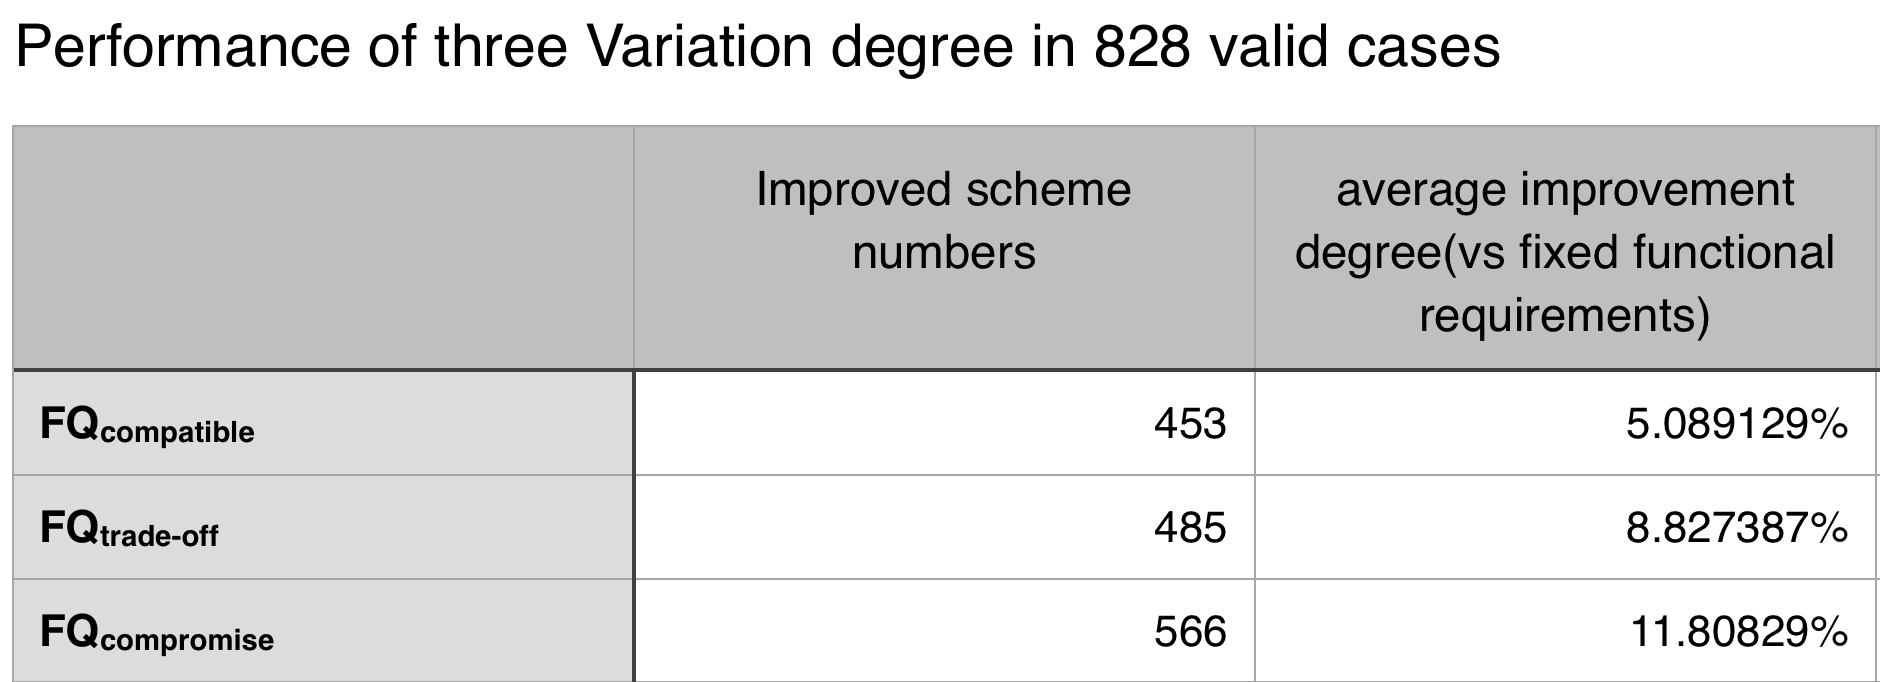
\includegraphics[width=13cm]{eval2-1.png}\]
%可以看\UTF{89C1}随着\UTF{5BF9}variation的程度的容忍度 \UTF{589E}加,越容易得到改\UTF{8FDB}方案,并且改\UTF{8FDB}方案的\UTF{8D28}量也会\UTF{589E}加,但同\UTF{65F6}探索空\UTF{95F4}也会相\UTF{5E94}地\UTF{589E}加。

%\[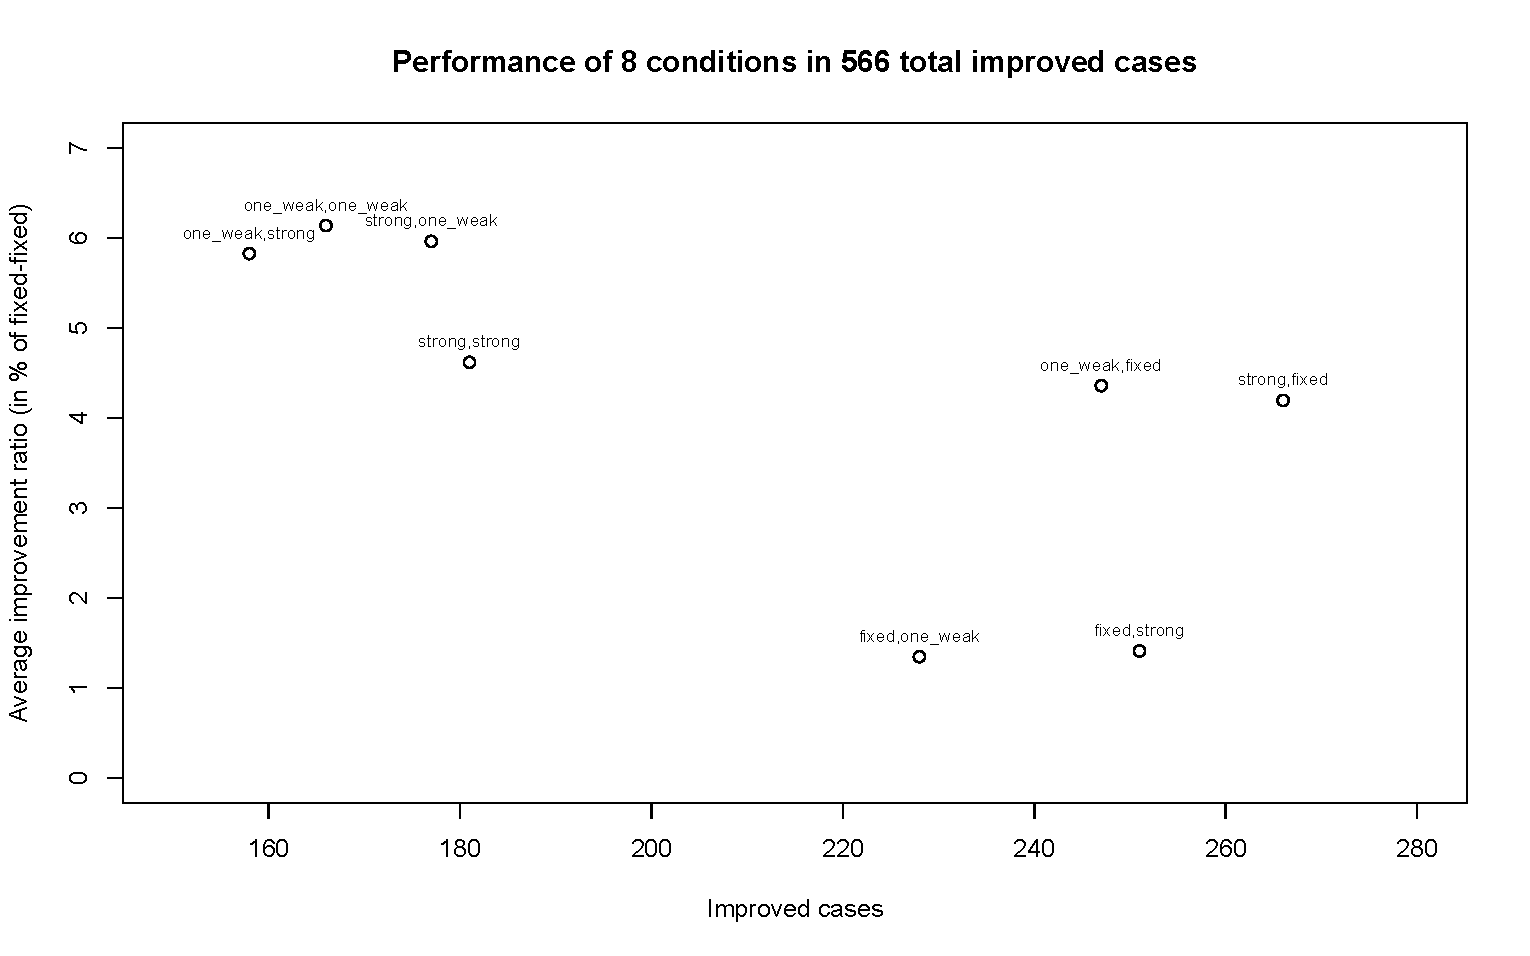
\includegraphics[width=13cm]{eval2.pdf}\]

\section{Algorithm}
Evaluation of Proposal 2\\
How fast can the proposed algorithm solve the extended problem?\\
Skyline vs Full search:\\
%step numbers: search from a service to a next service called one step
Fig. x depicts the relationship of step numbers and runtime between full search and skyline algorithm.
\[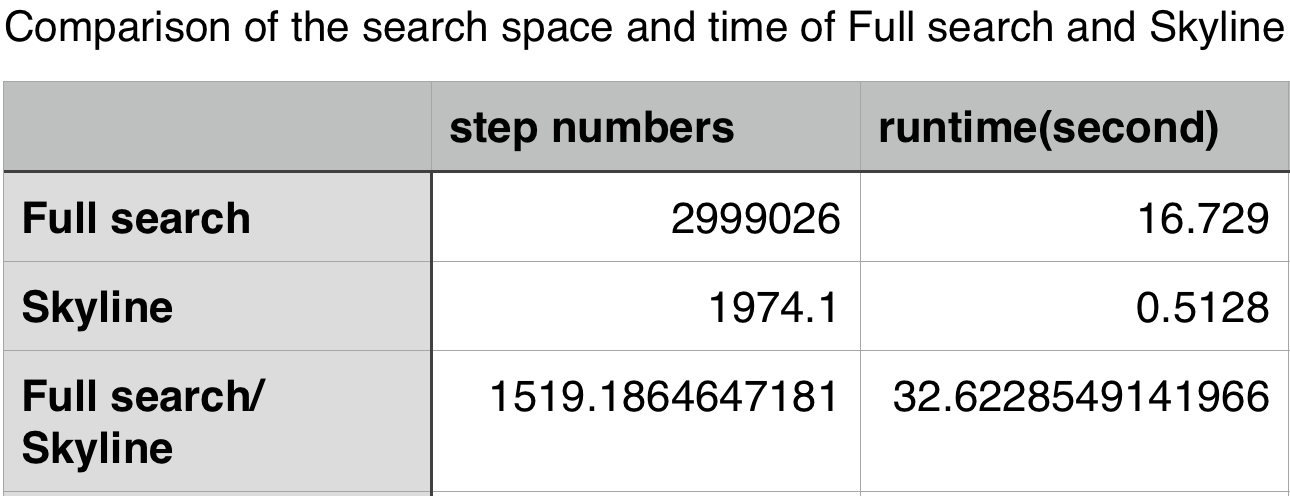
\includegraphics[width=13cm]{eval1.png}\]

%我\UTF{4EEC}可以看到step numbers 降到1/1519,\UTF{65F6}\UTF{95F4}降到了1/32.

- with skyline vs. proposed algorithm with skyline
\[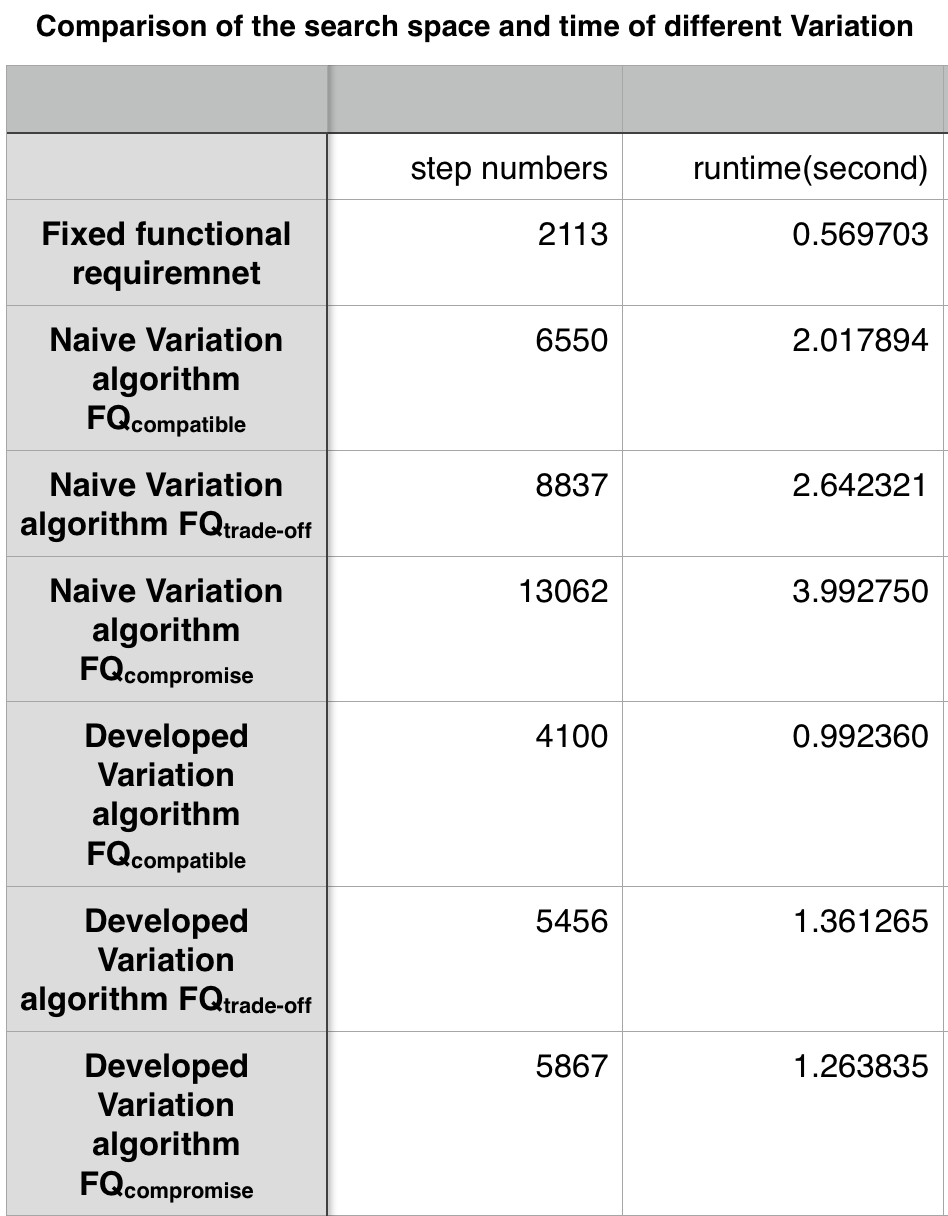
\includegraphics[width=13cm]{eval3.png}\]
%可以看\UTF{89C1}随着\UTF{5BF9}variation的程度的容忍度 \UTF{589E}加,\UTF{8BA1}算空\UTF{95F4}和\UTF{8BA1}算\UTF{65F6}\UTF{95F4}也会随之\UTF{589E}加。同\UTF{65F6}\UTF{5BF9}比相同variation degree的naive variation algorithm 和 developed variation algorithm可以得到,通\UTF{8FC7}算法的改\UTF{8FDB}可将\UTF{8FD0}行\UTF{65F6}\UTF{95F4}\UTF{7F29}短到原来的1/2到1/3,探索空\UTF{95F4}上也有的了不同程度的改\UTF{8FDB}。

\chapter{Discussion}
% related work can come here \UTF{626F}淡\UTF{5427}%

%我\UTF{4EEC}在section1中\UTF{8BA8}\UTF{8BBA}了Proposal,在section2中\UTF{8BA8}\UTF{8BBA}了Algorithm for Extended Composition Problem。

\section{Proposal}
%我\UTF{4EEC}在subsection1中\UTF{8BA8}\UTF{8BBA}了The extended problem should be significant because in the experiment
%在subsection2中\UTF{8BA8}\UTF{8BBA}了%The proposed algorithm made good improvement because in the experiment
\subsection{Extended Composition Problem}
%The extended problem should be significant because in the experiment

%根据\UTF{56FE}。。可以得到,改\UTF{8FDB}的\UTF{95EE}\UTF{9898}定\UTF{4E49}\UTF{663E}著地改\UTF{8FDB}了得到的方案的\UTF{8D28}量。其中FQ_compatible改\UTF{8FDB}了5.1%左右,FQ_trade-off改\UTF{8FDB}了8.8%左右,FQ_compromise改\UTF{8FDB}了11.8%左右,FQ_compromise改\UTF{8FDB}的幅度最大。同\UTF{65F6}\UTF{5BF9}比\UTF{56FE}。。中的fixed functional requirement 和 developed variation algorithm 中的three variation degree 的\UTF{8FD0}行\UTF{65F6}\UTF{95F4}   可以得到  ,后三者分\UTF{522B}要花前者的1.74,2.16,2.22倍的\UTF{8FD0}行\UTF{65F6}\UTF{95F4}。FQ_trade-off的改\UTF{8FDB}幅度比起FQ_compromise少了3%,\UTF{8FD0}行\UTF{65F6}\UTF{95F4}却基本一致,\UTF{8FD9}是由于\UTF{8FD9}\UTF{4E24}者的group数都是3 所\UTF{5BFC}致的。所以比起\UTF{9009}\UTF{62E9}FQ_trade-off,不如\UTF{9009}\UTF{62E9}FQ_compromise。那\UTF{4E48}是不是FQ_compromise就是最好的\UTF{5462}?我\UTF{4EEC}可以找到反例。\UTF{5B9E}\UTF{9645}上在intro中介\UTF{7ECD}的那个故事中,web seriver provider的目的是help user to rental a car for shopping,所以\UTF{9009}\UTF{62E9} 利用can seach any car的search engine s1,  和利用can only search kei car 的engine s2 都能\UTF{8FBE}到效果。如果provider的目的是help user to rental a car for clambing mountions的\UTF{8BDD},kei car的\UTF{9A6C}力很可能不能\UTF{8FBE}到爬山\UTF{8FD9}个目的。如果\UTF{8FD9}\UTF{65F6}候\UTF{9009}\UTF{62E9}用FQ_compatible的\UTF{8BDD},包含s2的workflow就会出\UTF{73B0}在scheme中,可\UTF{5B9E}\UTF{9645}上它是无法\UTF{8FBE}成目的的。\UTF{7EFC}上所\UTF{8BC9},FQ_compatible和FQ_compromise是\UTF{4E24}个可\UTF{9009}的\UTF{9009}\UTF{9879},FQ_compatible一定能\UTF{8FBE}成目的并且\UTF{8BA1}算\UTF{65F6}\UTF{95F4}快,但是得到的方案没FQ_compromise\UTF{8FD9}\UTF{4E48}好。FQ_compromise方案比FQ_compromise好,但是花\UTF{8D39}\UTF{65F6}\UTF{95F4}多,并且方案中的某些plan可能并不能\UTF{6EE1}足user的目的。到底\UTF{9009}\UTF{62E9}它\UTF{4EEC}中的\UTF{54EA}一个,\UTF{8FD8}需要user来决定。

\subsection{Algorithm for Extended Composition Problem}
%The proposed algorithm made good improvement because in the experiment

%如同在related中\UTF{5BF9}全探索所介\UTF{7ECD}的一\UTF{6837},全探索的探索空\UTF{95F4}是task内的services数 的 task\UTF{603B}数次方。skyline之后的探索空\UTF{95F4}是(select之后的task内的services数)^task\UTF{603B}数次方 。%我\UTF{4EEC}可以看到step numbers 降到1/1519。因\UTF{4E3A}有10个task,所以我\UTF{4EEC}推算可得,平均一个task中 select 剩下 不到 root 10 1519 \UTF{79CD}路径。而\UTF{65F6}\UTF{95F4}降到了1/32,并没有\UTF{8FD9}\UTF{4E48}\UTF{663E}著的下降。\UTF{8FD9}是由于\UTF{6BCF}一\UTF{6B65}都\UTF{989D}外\UTF{8FD0}行了select所\UTF{5BFC}致的。
%\UTF{5BF9}于figure。。中所有的行来\UTF{8BF4},探索\UTF{65F6}\UTF{95F4}和它\UTF{4EEC}的探索空\UTF{95F4}大致成正比,所以接下来我\UTF{4EEC}用探索空\UTF{95F4}来\UTF{5BF9}比naive variation algorithm和developed variation algorithm。\UTF{8FD0}用developed variation algorithm的FQcompatible 的探索空\UTF{95F4} \UTF{4EC5}\UTF{4EC5}\UTF{4E3A}\UTF{8FD0}用naive variation algorithm 0.625954198, 而\UTF{5BF9}于FQtrade-off 和 FQcompromise \UTF{8FD9}个\UTF{503C}\UTF{53D8}成了.617404096和.449165518。可以看\UTF{89C1},随着探索空\UTF{95F4}的\UTF{589E}加,developed variation algorithm比起naive variation algorithm\UTF{8282}省的探索空\UTF{95F4}和探索\UTF{65F6}\UTF{95F4}就越多。

\section{Future Work}
%本section我\UTF{4EEC}\UTF{8BA8}\UTF{8BBA}了本片\UTF{8BBA}文的不足和未来需要改\UTF{8FDB}的地方。
\subsection{QoS constraints}
%本文并没有\UTF{8BBE}定QoS constraints,\UTF{8FD9}在一定程度上\UTF{7B80}化了\UTF{95EE}\UTF{9898},方便了\UTF{8BA1}算,但是\UTF{4E3A}了将来\UTF{5E94}\UTF{5BF9}更\UTF{590D}\UTF{6742}更符合\UTF{5B9E}\UTF{9645}的service compostion problem,我\UTF{4EEC}需要\UTF{8FDB}一\UTF{6B65}改\UTF{8FDB}skyline算法。
\subsection{adaptive}
%本文的variation degree需要用\UTF{6237}自己\UTF{8BBE}定,将来可以考\UTF{8651}\UTF{8BA9}程序根据用\UTF{6237}的目的,自\UTF{52A8}感知出它所\UTF{5E94}\UTF{8BE5}取的variation degree
\subsection{change scability}
%本文\UTF{4E3A}了\UTF{8BA1}算方便将task\UTF{8BBE}定成10个,\UTF{6BCF}个task内的service\UTF{8BBE}定成10个。将来可以控制task个数\UTF{589E}加\UTF{6BCF}个task内的services数 ,或者 保持task内的service个数不\UTF{53D8},\UTF{589E}加task的\UTF{603B}数 \UTF{6D4B}\UTF{8BD5}其\UTF{6269}\UTF{5F20}性。\UTF{8FD8}可以将task中的service个数\UTF{8BBE}置成随机,看看不同情况的workflow template的表\UTF{73B0}怎\UTF{4E48}\UTF{6837}。

\chapter{Conclusion}

%由于在service合成\UTF{65F6},合成者的目的和他\UTF{8BBE}定的functional reqirement很\UTF{96BE}完全一致,并且\UTF{786E}\UTF{8BA4}它\UTF{4EEC}是否一致是很困\UTF{96BE}的,所以能\UTF{591F}\UTF{5E94}\UTF{5BF9}\UTF{8FD9}些困\UTF{96BE}的extended composition problem的出\UTF{73B0}就迫在眉睫。
%本文研究service composition,提出了一\UTF{79CD}新的composition problem的定\UTF{4E49},并\UTF{5BF9}解决它提出了算法,并展\UTF{5F00}了\UTF{4F18}化。并通\UTF{8FC7}\UTF{5B9E}\UTF{9A8C}\UTF{6D4B}\UTF{8BD5}出三\UTF{79CD}degree variation的探索空\UTF{95F4}和探索\UTF{65F6}\UTF{95F4},并\UTF{8FDB}行了\UTF{4F18}化。
%\UTF{5BF9}比他\UTF{4EEC},得出\UTF{7ED3}\UTF{8BBA}:
%FQ_trade-off的改\UTF{8FDB}幅度比起FQ_compromise少了3%,\UTF{8FD0}行\UTF{65F6}\UTF{95F4}却基本一致,\UTF{8FD9}是由于\UTF{8FD9}\UTF{4E24}者的group数都是3 所\UTF{5BFC}致的。所以比起\UTF{9009}\UTF{62E9}FQ_trade-off,不如\UTF{9009}\UTF{62E9}FQ_compromise。
%FQ_compatible一定能\UTF{8FBE}成目的并且\UTF{8BA1}算\UTF{65F6}\UTF{95F4}快,但是得到的方案没FQ_compromise\UTF{8FD9}\UTF{4E48}好。FQ_compromise方案比FQ_compromise好,但是花\UTF{8D39}\UTF{65F6}\UTF{95F4}多,并且方案中的某些plan可能并不能\UTF{6EE1}足user的目的。到底\UTF{9009}\UTF{62E9}它\UTF{4EEC}中的\UTF{54EA}一个,\UTF{8FD8}需要user来决定。


%-------------------
\bibliographystyle{plain} 
\bibliography{myref} 
%-------------------
\end{document}
